\documentclass[11pt,a4paper]{report}

\usepackage[margin=1.0in]{geometry}
\usepackage{polytechnique,url}
\usepackage{graphicx}
\usepackage{pdfpages}

\title{Specifications for the Attitude Control and Determination System-XCubeSat} 
\author{Dhruv Sharma, Damien Seux, Quentin Lisack, Kevin Garanger}

\date{12 April 2015} 

\renewcommand{\titrecourt}{Specifications ADCS}
\setcounter{secnumdepth}{5}
\begin{document}
\maketitle

\tableofcontents

\chapter{Introduction}

The objective of this document is to summarize in one place the specifications related to the software of the Attitude Control and Determination System, henceforth ADCS of the nano-satellite X-CubeSat developed by the students of École Polytechnique, Paris. We have divided the document into the following sections 

\begin{itemize}
\item 
Definition of the architecture of the ADCS 
\item 
External Interfaces available on the ADCS 
\item 
Sensors and peripherals on the ADCS 
\item 
Data formats used for computing 
\item 
Protocols for testing 
\end{itemize}

This document shall be useful for all people currently concerned with the conception of the ADCS and eventually for students who will take over the project in the months to come. This document is however, far from being complete and additions, corrections and deletions will be made till the day of delivery. 

\chapter{Architecture of the ADCS}\thispagestyle{fancy}

The ADCS uses a microprocessor manufactured by ST Microelectronics based on the ARM Cortex-M4 Architecture. The model used is STM 32F405 RGT6

The available interfaces, sensors and other peripherals available on the ADCS are: 

\begin{itemize}
\item 
32 MB External Memory  
\item 
7(or 9) sun sensors 
\item 
Magnetometer
\item 
Gyrometer
\item 
H-Bridges to modulate power to the magneto-torquers 
\item 
A Serial interface with the On-Board Computer (\textit{Ordinateur de Bord} henceforth, ODB) 
\end{itemize}

Following is the complete plan for the ADCS: 

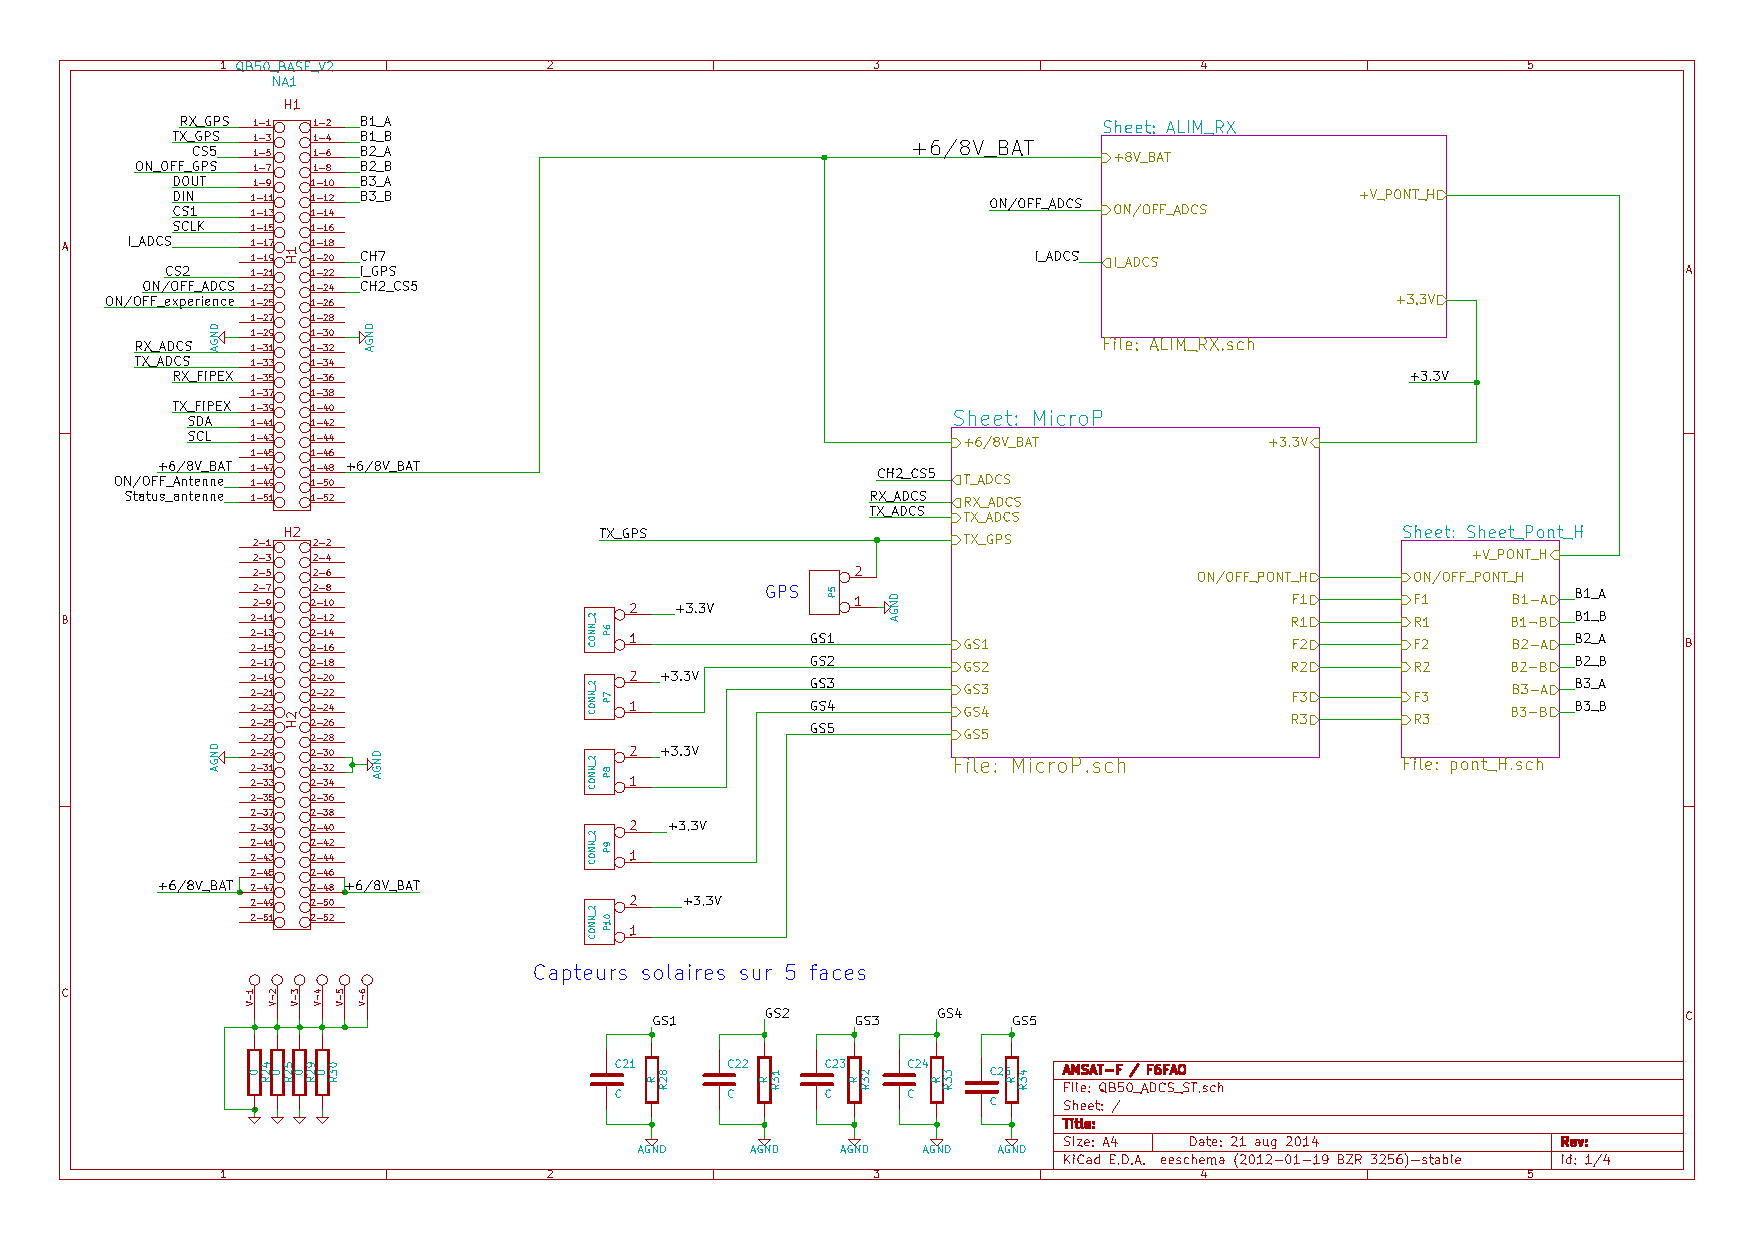
\includepdf[pages={-},angle=90]{QB50_ADCS_ST.pdf}

\chapter{External interfaces} \thispagestyle{fancy}

\chapter{Sensors and peripherals} \thispagestyle{fancy}

\chapter{Data formats}\thispagestyle{fancy}

\chapter{Testing}\thispagestyle{fancy} 


\end{document}